\documentclass{article}
\usepackage{geometry}
 \geometry{
 a4paper,
 total={170mm,257mm},
 left=20mm,
 top=20mm,
 }
\usepackage{graphicx}
\usepackage{hyperref}
\usepackage{biblatex}
\usepackage{amsmath,amssymb}
\usepackage{subcaption}
\usepackage{neuralnetwork}
\usetikzlibrary{positioning}

\addbibresource{sources.bib}

\author{Meftah, Morteza M.D; Waren, Daniel M.D; Bosco, Joseph A. IV;\\
Di Gangi, Catherine; Watson, Cody Ph.D}
\title{Modeling Robotic Surgery Predictions: Write-Up}

\begin{document}

\tikzset{%
  every neuron/.style={
    circle,
    draw,
    minimum size=1cm
  },
  neuron missing/.style={
    draw=none, 
    scale=4,
    text height=0.333cm,
    execute at begin node=\color{black}$\vdots$
  },
}

\newcommand\epochs{86}
\newcommand\batchsize{4}
\newcommand\convergence{6}
\newcommand\mse{1.819}
\newcommand\ns{0.587}

\maketitle

\textbf{%
DISCLAIMER:
This is a VERY rough draft of the write-up. 
It is meant to demonstrate the work I have done on the project in a way that you don't need to read any code.
Document written by Jack Bosco. 
Code for the data analysis, modeling, and visualization are also written by Jack Bosco. 
}

\section{Methods}

Overview

	Analysis of pre-operative planning and report screenings from 626 TKR cases
was used to establish the NYU method for approximating optimal post-resection tibial
and femoral coronal alignments based on the pre-operative tibial and femoral coronal alignments.
To establish a unified input format, femoral and tibial coronal alignments are translated into MPTA and LDFA measurements, respectively.
MPTA and LDFA were chosen since they allow for easy computation of aHKA and JLO values to visualize the knee morphology through CPAK classification \cite{cpak-paper}.
After calculating the measurements, MPTA and LDFA values are fed into a min-max scaler transformation to normalize the input and output values within the range [-1, 1] \cite{mm-norm}.
The last pretraining step splits the normalized data into testing, training and validation sets of sizes 30\%, 66.5\% and 3.5\% respectively with random seed 42.
In training the model runs stochastic gradient descent, looping until a maximum number of repetitions is reached or 10 repetitions are completed with no change in error.
After it is finished training, the model is evaluated using the mean squared error between the de-normalized predicted aHKA and target aHKA values from the testing dataset.

Pre-Processing

	The pre-processing step involves all the actions performed on the raw dataset before the model can be trained.
In this experiment, tibial and femoral coronal alignments of the knee region are translated into MPTA and LDFA measurements, respectively.
The MPTA measurement is a representation of the tibial coronal alignment such that perfectly aligned tibial coronal angles map to 90° 
and the equations $\text{aHKA}=\text{MPTA}-\text{LDFA}$ and $\text{JLO}=\text{MPTA}+\text{LDFA}$ satisfy the CPAK morphologies defined by \cite{cpak-paper}.
Similarly, the LDFA measurement is a representation of the femoral coronal alignment such that perfectly aligned femoral coronal angles map to 90°
and the equations $\text{aHKA}=\text{MPTA}-\text{LDFA}$ and $\text{JLO}=\text{MPTA}+\text{LDFA}$ give the CPAK morphologies defined by MacDessi et. al.\cite{cpak-paper}.
For the input space $X$, pre-operative MPTA and LDFA angles are combined into vectors $x_i=[\text{preop MPTA}_i, \text{preop LDFA}_i]$
where $i$ denotes the REDCAP ID number. The same is done for the output space $Y: y_i=[\text{planned MPTA}_i, \text{planned LDFA}_i]$.
To train and evaluate the model, we split the input and output data into testing, training and validation sets of sizes 30\%, 66.5\% and 3.5\% respectively.
Each split contains an equal number of pre-op and planned values, linked by case through the REDCAP ID.

	Next, two normalizers are defined: $\text{norm}_Y$ and $\text{norm}_Y$.
They use the min max scaler algorithm defined in the scikit-learn library \cite{scikit-learn} to normalize the values of the input and output
by scaling them within the range [-1, 1].
$\text{norm}_x$ is fitted to the training subset of $X$, $norm_Y$ is fitted to the training subset of $Y$.
After fitting, the normalizer coefficients are saved so that individual [MPTA, LDFA] samples can be normalized and de-normalized deterministically.

Training

\begin{figure}[ht]
	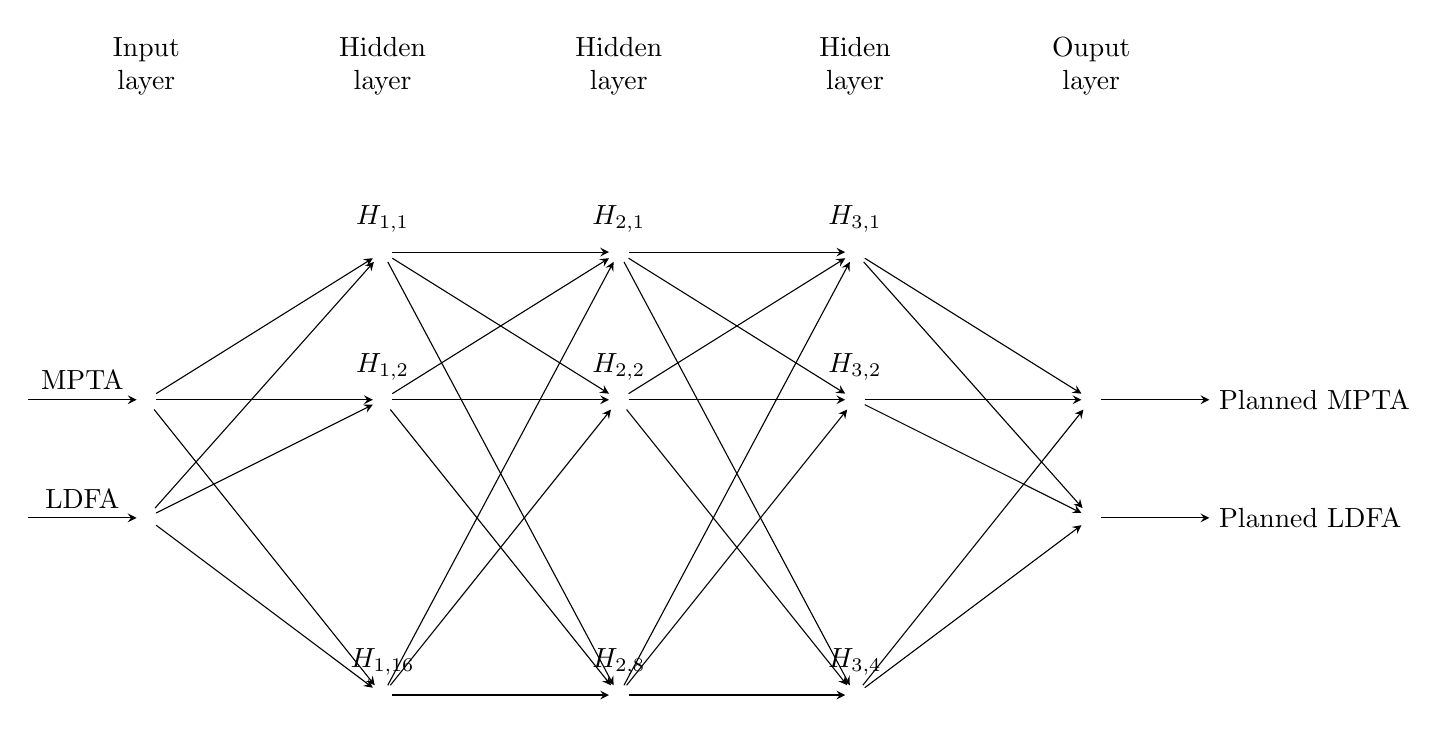
\begin{tikzpicture}[x=1.5cm, y=1.5cm, >=stealth]
		\foreach \m/\l [count=\y] in {1,2}
		\node [every neuron/.try, neuron \m/.try] (input-\m) at (0,.5-\y) {};

		\foreach \m [count=\y] in {1,2,missing,3}
		\node [every neuron/.try, neuron \m/.try ] (hidden1-\m) at (2,2-\y*1.25) {};

		\foreach \m [count=\y] in {1,2,missing,3}
		\node [every neuron/.try, neuron \m/.try ] (hidden2-\m) at (4,2-\y*1.25) {};

		\foreach \m [count=\y] in {1,2,missing,3}
		\node [every neuron/.try, neuron \m/.try ] (hidden3-\m) at (6,2-\y*1.25) {};

		\foreach \m [count=\y] in {1,2}
		\node [every neuron/.try, neuron \m/.try ] (output-\m) at (8,.5-\y) {};

		\draw [<-] (input-1) -- ++(-1,0) node [above, midway] {MPTA};
		\draw [<-] (input-2) -- ++(-1,0) node [above, midway] {LDFA};

		\foreach \j in {1,2,3}{
			\foreach \l [count=\i] in {1,2}
			\node [above] at (hidden\j-\i.north) {$H_{\j,\l}$};
		}
		\node [above] at (hidden1-3.north) {$H_{1,16}$};
		\node [above] at (hidden2-3.north) {$H_{2,8}$};
		\node [above] at (hidden3-3.north) {$H_{3,4}$};

		\draw [->] (output-1) -- ++(1,0) node [above, right] {Planned MPTA};
		\draw [->] (output-2) -- ++(1,0) node [above, right] {Planned LDFA};

		\foreach \i in {1,...,2}{
			\foreach \j in {1,...,3}
				\draw [->] (input-\i) -- (hidden1-\j);
		}

		\foreach \i in {1,...,3}{
			\foreach \j in {1,...,3}
				\draw [->] (hidden1-\i) -- (hidden2-\j);
		}
		
		\foreach \i in {1,...,3}{
			\foreach \j in {1,...,3}
				\draw [->] (hidden2-\i) -- (hidden3-\j);
		}

		\foreach \i in {1,...,3}
		\foreach \j in {1,...,2}
			\draw [->] (hidden3-\i) -- (output-\j);

		\foreach \l [count=\x from 0] in {Input, Hidden, Hidden, Hiden, Ouput}
		\node [align=center, above] at (\x*2,2) {\l \\ layer};

	\end{tikzpicture}
	\caption{Diagram of the MLP model architecture}
	\label{fig:mlp_diagram}
\end{figure}

	For the NYU method a multilayer perceptron (MLP) model, also known as a neural network, is trained to determine the regression line of best fit \cite{mlp-paper}.
An MLP architecture for the model was chosen based on the following factors: the size of the dataset, the input dimensions and the output dimensions.
Since the size of the dataset is small (626 cases), a more robust deep learning architecture is not an option.
The MLP architecture we used had three hidden layers of sizes 16, 8 and 4 (Figure \ref{fig:mlp_diagram}),
making it large enough to learn feature representations of the input and small enough to converge on a small sample size \cite{deep-learning-paper}.
We used stochastic gradient descent as the optimizer, set the random seed to 42, and used hyperbolic tangent as our activation function since its range (-1,1)
fits well within the range of the normalizer [-1,1] \cite{sgd-paper, mlp-paper}.
Other hyperparameters are set to their default value as per the scikit-learn documentation \cite{sklearn-sgd, adaptive-lr, scikit-learn, momentum-paper}.
The input dimension (2) and output dimension (2) disqualified the option of using traditional support vector machines for this model.
Multi-output SVM regressors are an option, however these work by combining two separate regressors \cite{svm-paper},
one to predict MPTA and one to predict LDFA, and would therefore blind to the relationship between pre-operative and post-operative aHKA values. 

Evaluation

	To measure the accuracy of the model we calculated and compared the aHKA values for pre-operative and planned knee alignments.
To do so, we first took the following difference between non-normalized MPTA and LDFA patterns within the testing sets: 
$X_\text{test}$, $Y_\text{test}$: 
$$X_\text{test, aHKA}=\{\text{MPTA} - \text{LDFA} | [\text{MPTA}, \text{LDFA}] \in X_\text{test}\}$$
$$Y_\text{test, aHKA}=\{\text{MPTA} - \text{LDFA} | [\text{MPTA}, \text{LDFA}] \in Y_\text{test}\}$$
Then the model predicts planned LDFA and MPTA values in the testing set ($Y_\text{pred}$). 
The model predicts the normalized the input ($\text{norm}_x(x_i)$), running the normalized input through the model ($\text{predict}(\text{norm}_x(x_i))$),
and de-normalizing the predicted planned alignmnets ($\text{norm}_y^{-1}$):
$$Y_\text{pred}=\{\text{norm}_y^{-1}(\text{predict}(\text{norm}_x(x_i))) | x_i \in X_\text{test}\}$$
To compare our predictions with $Y_\text{test, aHKA}$, we evaluate $Y_\text{pred, aHKA}$ in the same manner as $Y_\text{test, aHKA}$: 
$$Y_\text{pred, aHKA}=\{\text{MPTA} - \text{LDFA} | [\text{MPTA}, \text{LDFA}] \in Y_\text{test}\}$$
Since the testing set is split from the training set the model has never seen the patterns in $X_\text{test}$ or $Y_\text{test}$ before.
By doing so, we get a preliminary understanding of how this model may perform in the field.
As the final step, we take the mean squared error between the targets $Y_\text{test, aHKA}$ and the predictions $Y_\text{pred, aHKA}$ to evaluate the model's accuracy.

	
\section{Results}

\begin{figure}[h]
	\begin{subfigure}{.45\linewidth}
		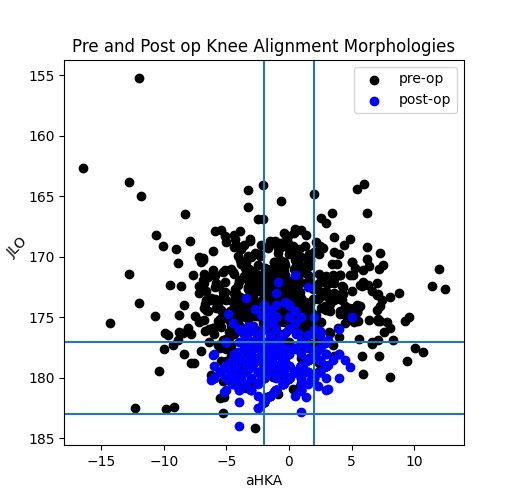
\includegraphics[width=\linewidth]{data_vis.png}
		\caption{Pre-op vs. Planned value distributions showing CPAK morpholigies.}
		\label{data_vis}
	\end{subfigure}
	\hfill
	\begin{subfigure}{.45\linewidth}
		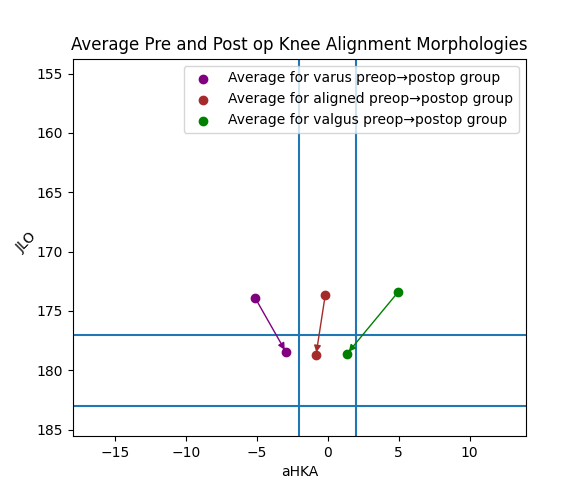
\includegraphics[width=\linewidth]{avg_vis.png}
		\caption{Average change from pre-op to planning stage by aHKA morphology}
		\label{avg_vis}
	\end{subfigure}
	\caption{Visualization of dataset}
\end{figure}

Training
	The model converged early, halting after training for \epochs with a batch size of \batchsize patterns (Figure \ref{loss_curve}).
After about \convergence epochs, the mean squared error between normalized input/target patterns begins to converge.
The model takes less than 1 minute to converge with no GPU, however it is important to note this is with a small training set of 417 patterns.
Nonetheless, with the simple feed-forward neural net architecture chosen for this model, it is expected that the model will train relatively quickly. 

\begin{figure}[h!]
	\centering
	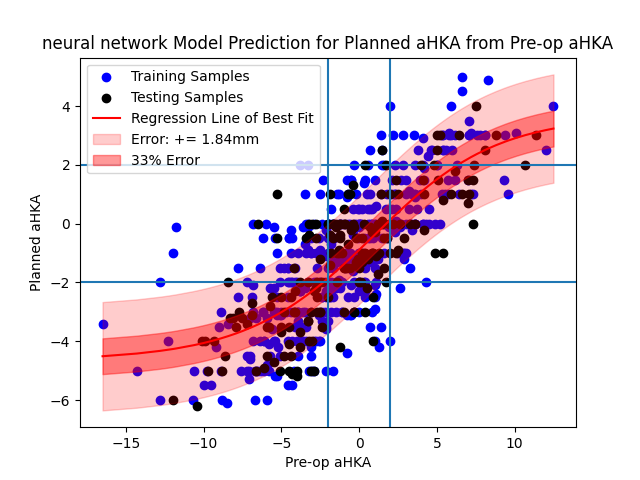
\includegraphics[width=.65\linewidth]{neural_network_regression.png}
	\caption{Visualization of the regression line of best fit produced by the MLP model}
	\label{regression}
\end{figure}

\begin{figure}[h!]
	\centering
	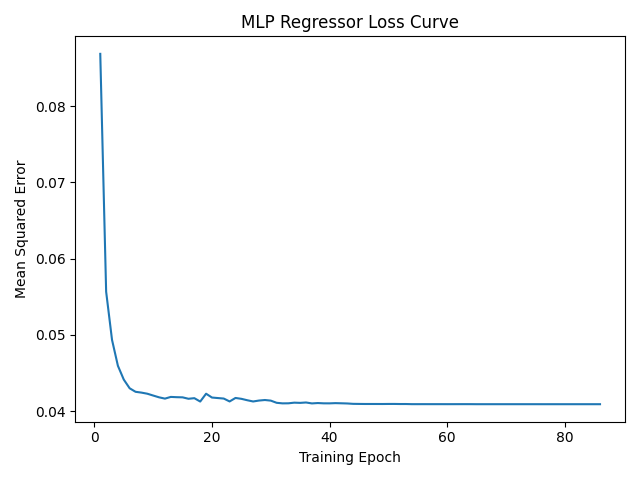
\includegraphics[width=.5\linewidth]{loss_curve.png}
	\caption{Loss curve for the MLP training. Mean squared error is shown for each epoch (\batchsize \space repitions) from the normalized prediction/target patterns.}
	\label{loss_curve}
\end{figure}

Shape

	The regression this model produces is in-line with the hypothesized change in pre-op to planned aHKA.
In Figure \ref{data_vis}, the pre-operative and post-operative aHKA and JLO values from the initial dataset are shown.
The pre-operative values were more varied than their planned counterparts and the vertical and horizontal bars separate the different knee alignment morphologies \cite{cpak-paper}.
Splitting the pre-operative values by aHKA into varus, valgus and aligned groups, we can view the average change for each group from pre-op to planning stage (Figure \ref{avg_vis}).
For each group, the JLO tends to move in the same direction. More interestingly, however, is the way aHKA changes by group: 
on average, varus morphologies tend to stay varus and aligned morphologies tend to stay aligned but valgus morphologies are planned to be corrected to aligned morphologies.
Looking at the regression produced from the model (Figure \ref{regression}), we see the same pattern.
Blue dots represent the training and validation set while block dots represent the testing set.
The middle-left square is hardly intersected by the regression, indicating the model rarely predicts aligned morphologies from varus morphologies.
The middle-right square is intersected by the regression, however, indicating the model sometimes predicts aligned morephologies from valgus morphologies.

Accuracy

	Evaluative statistics demonstrate the NYU method for planning knee morphologies is more accurate than making predictions about the mean
(RMSE \mse; Nash Sutcliffe \ns) \cite{goodness-of-fit}. 
As the regression (Figure \ref{regression}) moves towards more densely populated regions of the scatter plot, the line of best straightens out.
This demonstrates how the model successfully avoids overfitting so long as there are enough examples in the dataset.

Moving Forward

\begin{figure}[h]
	\centering
	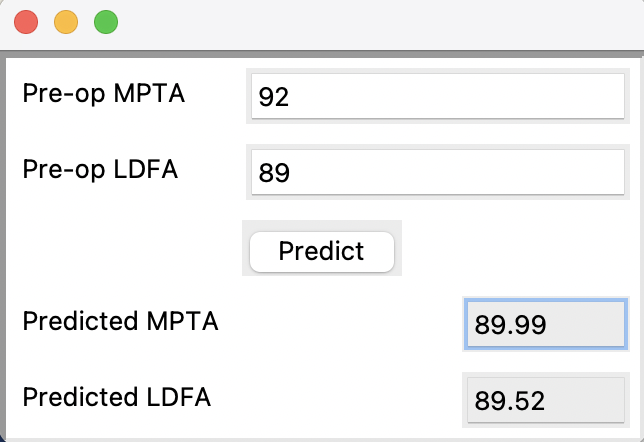
\includegraphics[width=.5\linewidth]{gui.png}
	\caption{Graphical User Interface (GUI) with example prediction}
	\label{gui}
\end{figure}

	More work needs to be done to evaluate the NYU methods usefulness for planning robotic TKR in the field.
Included in this study is a codebase from which the model can be trained if suppliad appropriate data. With a pre-trained model,
the NYU method is accessible through a graphical user interface (Figure \ref{gui}).
The GUI is brought up by running the gui.py script with a pre-trained model in the appropriate folder.
With it, the NYU method can be utilized without any code.

\medskip

\printbibliography

\end{document}

